%%%%%%%%%%%%%%%%%%%%%%%%%%%%%%%%%%%%%%%%%%%%%%%%%%%%%%%%%%%%
%%  This Beamer template was created by Cameron Bracken.
%%  Anyone can freely use or modify it for any purpose
%%  without attribution.
%%
%%  Last Modified: January 9, 2009
%%

\documentclass[xcolor=x11names,compress]{beamer}
%\documentclass[xcolor=x11names,compress,handout]{beamer} % ignores pauses

\xdefinecolor{orange}{rgb}{1,0.45,0}
\xdefinecolor{green}{rgb}{0,0.35,0}
\definecolor{blue}{rgb}{0.12,0.46,0.99} % crayola blue
\definecolor{gray}{rgb}{0.2,0.2,0.2} % dark gray

\xdefinecolor{cerulean}{rgb}{0.01,0.48,0.65}
\xdefinecolor{ust-blue}{rgb}{0,0.20,0.47}
\xdefinecolor{ust-mustard}{rgb}{0.67,0.52,0.13}

%% General document %%%%%%%%%%%%%%%%%%%%%%%%%%%%%%%%%%
\usepackage{graphicx}
\usepackage{multimedia}
\usepackage{tikz}
\usepackage[font=tiny,labelfont=bf]{caption}
\usetikzlibrary{intersections,shapes.arrows}
%\usepackage{tikz}
%\usetikzlibrary{decorations.fractals}
%%%%%%%%%%%%%%%%%%%%%%%%%%%%%%%%%%%%%%%%%%%%%%%%%%%%%%


%% Beamer Layout %%%%%%%%%%%%%%%%%%%%%%%%%%%%%%%%%%
\useoutertheme[subsection=false,shadow]{miniframes}
\useinnertheme{default}
\usefonttheme{serif}
\usepackage{palatino}
\usepackage{overpic}
\usepackage{empheq}

\setbeamerfont{title like}{shape=\scshape}
%\setbeamerfont{frametitle}{shape=\scshape}

\setbeamercolor*{lower separation line head}{bg=ust-blue} 
\setbeamercolor*{normal text}{fg=black,bg=white} 
\setbeamercolor*{alerted text}{fg=red} 
\setbeamercolor*{example text}{fg=black} 
%\setbeamercolor*{structure}{fg=black}
\setbeamercolor{title}{fg=ust-blue}
\setbeamercolor{frametitle}{fg=ust-blue}
\setbeamercolor*{structure}{fg=ust-mustard}  
 
\setbeamercolor*{palette tertiary}{fg=black,bg=black!10} 
\setbeamercolor*{palette quaternary}{fg=black,bg=black!10} 

%\setbeamercovered{transparent}

\newcommand{\highlight}[1]{\mathchoice%
  {\colorbox{black!10}{$\displaystyle#1$}}%
  {\colorbox{black!10}{$\textstyle#1$}}%
  {\colorbox{black!10}{$\scriptstyle#1$}}%
  {\colorbox{black!10}{$\scriptscriptstyle#1$}}}%

%\newcommand{\highlight}[1]{\colorbox{black!10}{\ensuremath{#1}}}
\renewcommand{\(}{\begin{columns}}
\renewcommand{\)}{\end{columns}}
\newcommand{\<}[1]{\begin{column}{#1}}
\renewcommand{\>}{\end{column}}

%\newcommand{\credit}[1]{\vskip0pt plus 1filll #1}
%%%%%%%%%%%%%%%%%%%%%%%%%%%%%%%%%%%%%%%%%%%%%%%%%%



%%%%%%%%%%%%%%%%%%%%%%%%%%%%%%%%%%%%%%%%%%%%%%%%%%%%%%%%%%%%%%
\title{{\tiny basic} Intro to Machine Learning}
\author%[Author, Another] % (optional, use only with lots of authors)
{}
\subtitle{\vspace*{5mm} 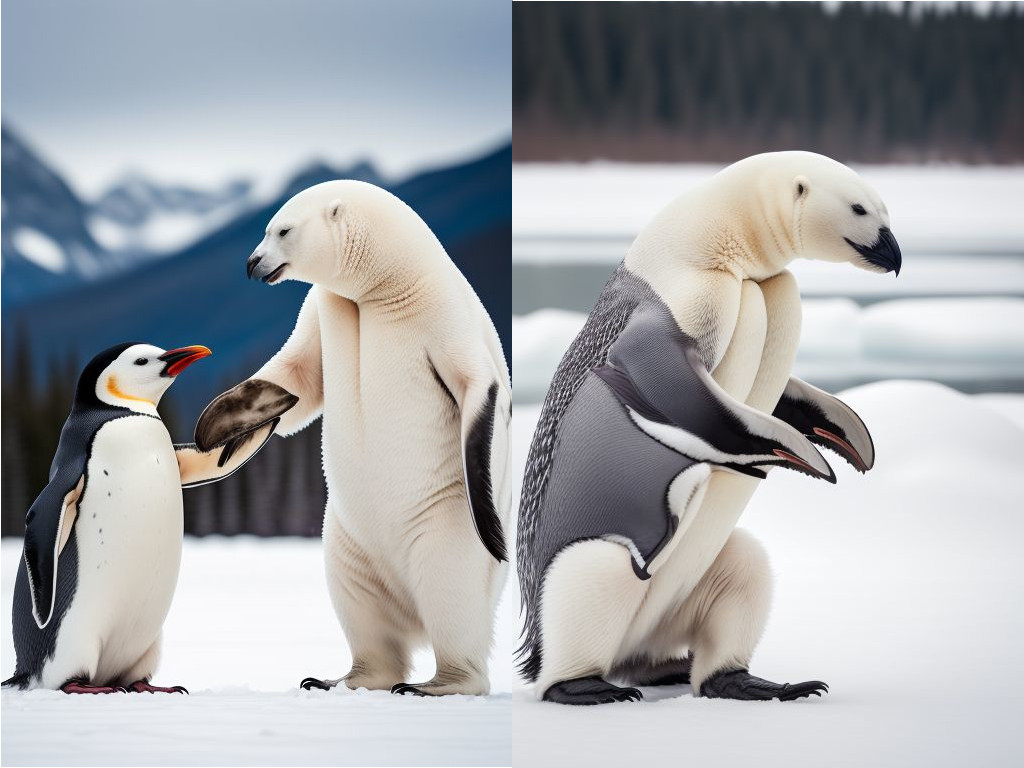
\includegraphics[width=0.7\textwidth]{penguinbear}}

\date{}

\begin{document}

\maketitle

% ------------------------------------------------------------------------------

\begin{frame}{Outline}

{\scriptsize (Just overview here; for actual content see Jupyter notebooks)}

\begin{itemize}
  \item a very loose introduction to Machine Learning (ML)
  \item[] $\to$ as a problem in regression / optimisation
  \item[] $\to$ supervised vs. unsupervised
  \item[] $\to$ sample usage in oceanography
  \item[]
  \item example with \structure{argo} data
  \item[] $\to$ what is Argo?
  \item[] $\to$ unsupervised ML example: clustering analysis
  \item[] $\to$ supervised ML example: neural networks
\end{itemize}

\end{frame}

% ------------------------------------------------------------------------------

\begin{frame}{Some propaganda to start with}

\parbox{0.5\textwidth}{ML algorithms are:
\begin{itemize}
  \item algorithms + tools, and that's it
  \item[] $\to$ very powerful, but context dependent
  \item usually \structure{black box}
  \item[] $\to$ it can work wonderfully / fail spectacularly, but you don't
  necessarily know why...
  \item[]
  \item[!!!] prudent to do sanity checks!
\end{itemize}}\hspace*{1mm}\parbox{0.45\textwidth}{\begin{figure}
  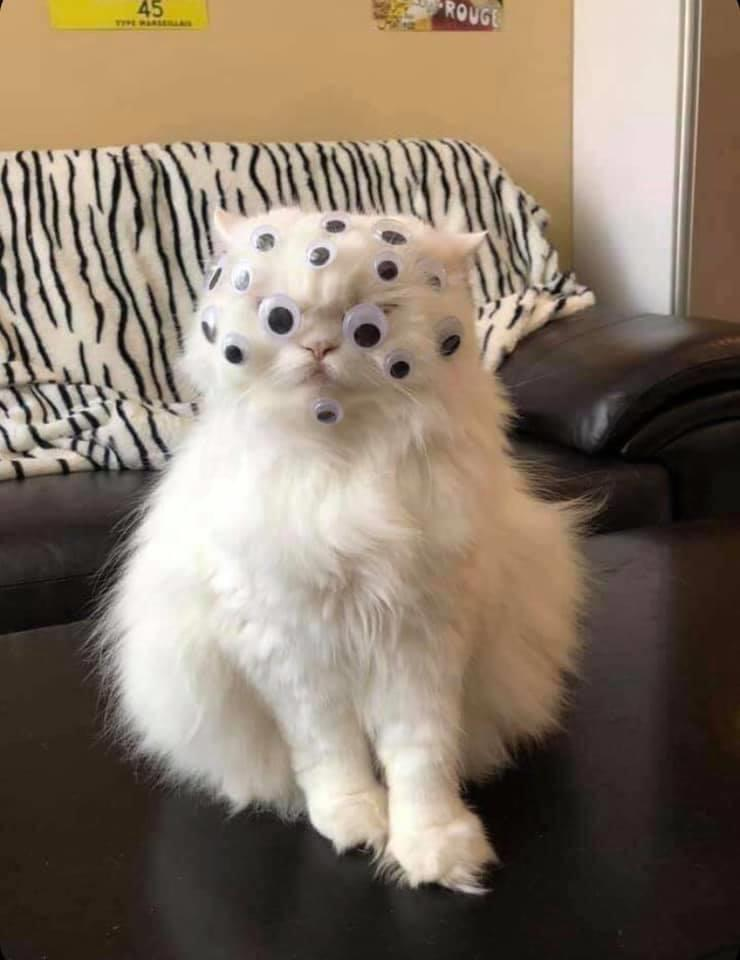
\includegraphics[width=0.45\textwidth]{cursed}
  \caption{Hermeowus Mora, disciple of Hermaeus Mora the Daedric prince of
  knowledge and memory}
\end{figure}}

\end{frame}

% ------------------------------------------------------------------------------

\begin{frame}{Cursed example: image recognition/generation}

\begin{figure}
  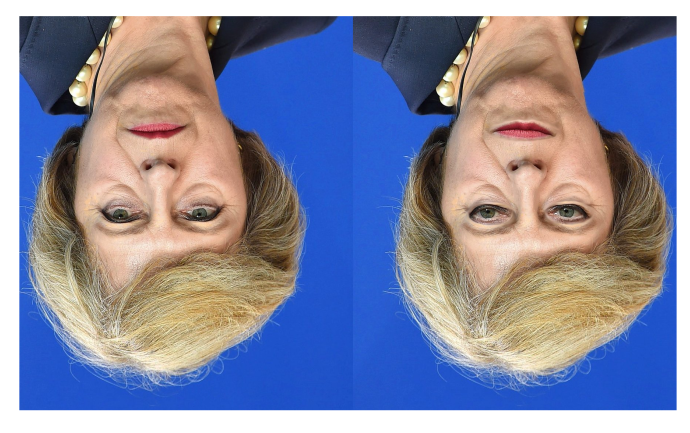
\includegraphics[width=\textwidth]{cursed_1}
\end{figure}

\end{frame}

% ------------------------------------------------------------------------------

\begin{frame}{Cursed example: image recognition/generation}

\begin{figure}
  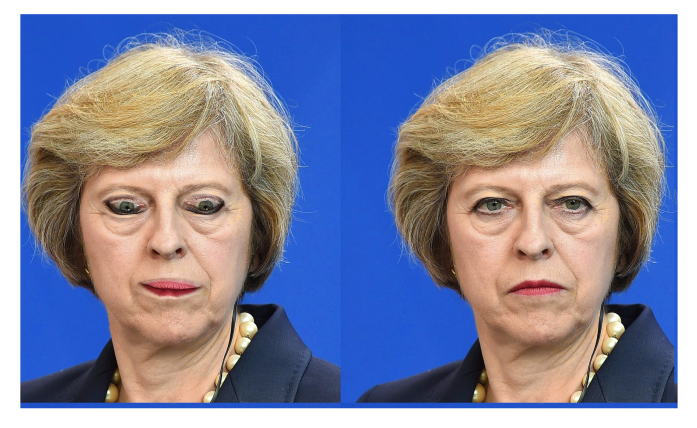
\includegraphics[width=\textwidth]{cursed_2}
\end{figure}

\end{frame}

% ------------------------------------------------------------------------------

\begin{frame}{Machine learning + regression/optimisation}

Recall that, in \structure{regression}, for $X$ the input, $Y$ the output, $f$ the model, where
\begin{equation*}
    Y = f(X),
\end{equation*}
the aim is to seek $f$ such that we minimise something like
\begin{equation*}
    J = \sum_i (Y_i - f(X_i))^2
\end{equation*}
\begin{itemize}
  \item[] $\to$ e.g. \structure{linear regression}, polynomial fitting
  \item[]
  \item ML in a nutshell follows the same principle
  \item[] $\to$ algorithms are different (e.g. nonlinear, network based,
  different optimiser, stochastic/probabilistic)
\end{itemize}

\end{frame}

% ------------------------------------------------------------------------------

\begin{frame}{Training, Validation, Testing data}

Normally split $(X, y)$ into
\begin{itemize}
  \item \structure{training data} ($X_{\rm train}, Y_{\rm train}$) {\tiny (most
  data should be here)}
  \item[] $\to$ exposed to ML algorithms for training the model
  \item[] $\to$ used to compute misfits or \structure{loss function}
  \item \structure{validation data} ($X_{\rm val}, Y_{\rm val}$)
  \item[] $\to$ exposed to ML algorithms to tune model
  \structure{hyperparameters} and/or model selection
  \item \structure{test data} ($X_{\rm test}, Y_{\rm test}$)
  \item[] $\to$ \textbf{NOT} exposed to ML algorithm
  \item[] $\to$ used to test performance of model
  \item[]
  \item[!!!] sometimes ``validation'' and ``test'' are swapped
\end{itemize}

\end{frame}

% ------------------------------------------------------------------------------

\begin{frame}{Unsupervised vs. supervised}

\begin{itemize}
  \item \structure{unsupervised} ML is where data is \structure{unlabelled}, and
  algorithm picks out features by themselves
  \item[] $\to$ e.g. PCA (so EOFs), clustering, some examples of neural networks
\end{itemize}

\begin{figure}
  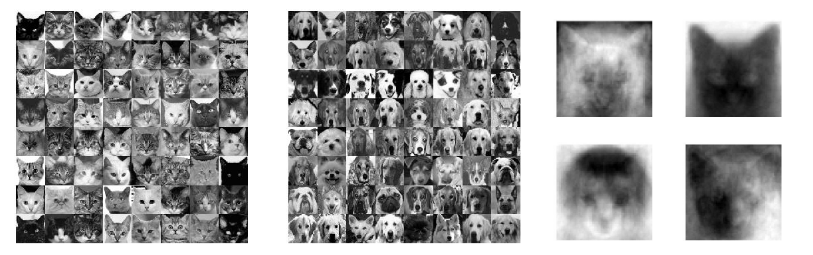
\includegraphics[width=\textwidth]{brunton_et_al_2013}
  \caption{Cursed cats/dogs (?) from PCA. Figure adapted from Fig. 10 of
  Brunton, Brunton, Proctor \& Kutz (2013).}
\end{figure}

\end{frame}

% ------------------------------------------------------------------------------

\begin{frame}{Unsupervised vs. supervised}

\begin{itemize}
  \item \structure{supervised} ML is where data is \structure{labelled}, and
  algorithm fits model between input and output
  \item[] $\to$ often want this for prediction purposes
  \item[] $\to$ e.g. (multi-)linear regression, some examples of neural networks
  \item[]
  \item other characterisations (e.g. \structure{semi-supervised},
  \structure{reinforcement})
\end{itemize}

\end{frame}

% ------------------------------------------------------------------------------

\begin{frame}{Unsupervised vs. supervised}

\begin{figure}
  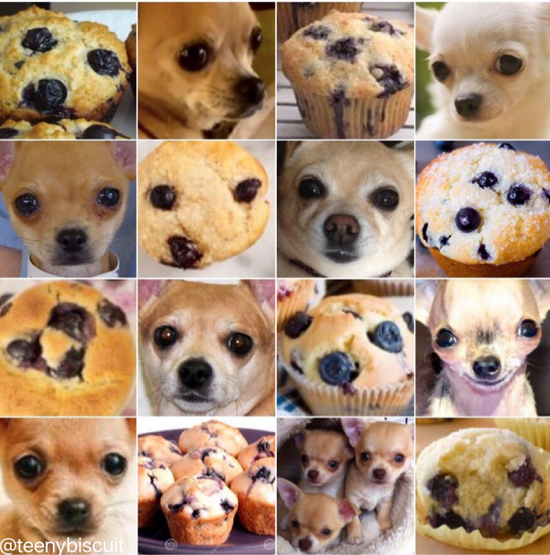
\includegraphics[width=0.48\textwidth]{muffin}\hspace*{1mm}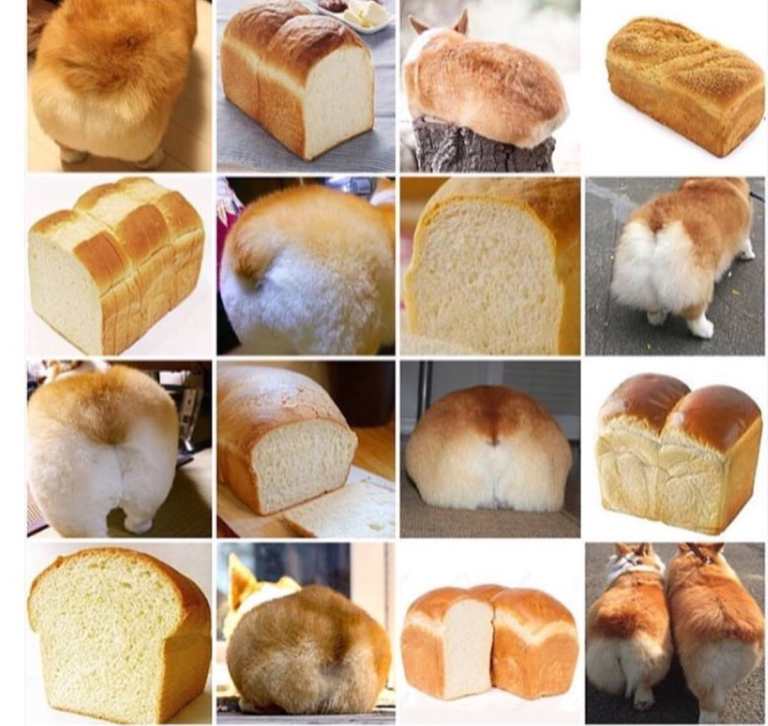
\includegraphics[width=0.51\textwidth]{bread}
  \caption{Various entries from the ``animal or things'' meme, as found on the
  internet.}
\end{figure}

\end{frame}

% ------------------------------------------------------------------------------

\begin{frame}{Unsupervised vs. supervised}

\begin{figure}
  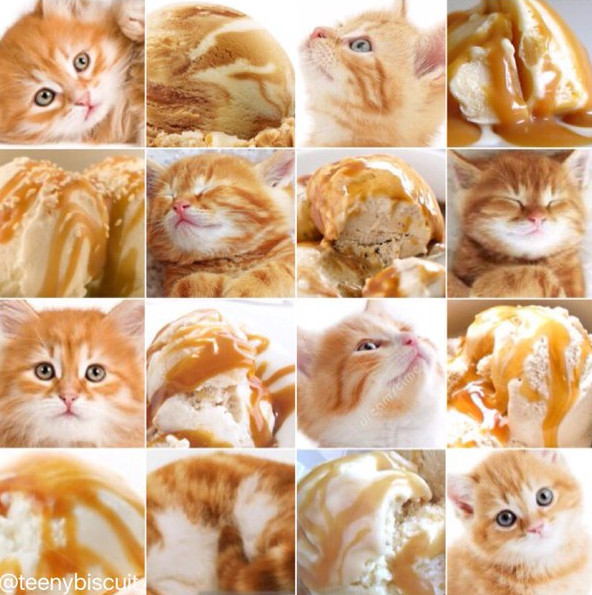
\includegraphics[width=0.3\textwidth]{ice_cream_2}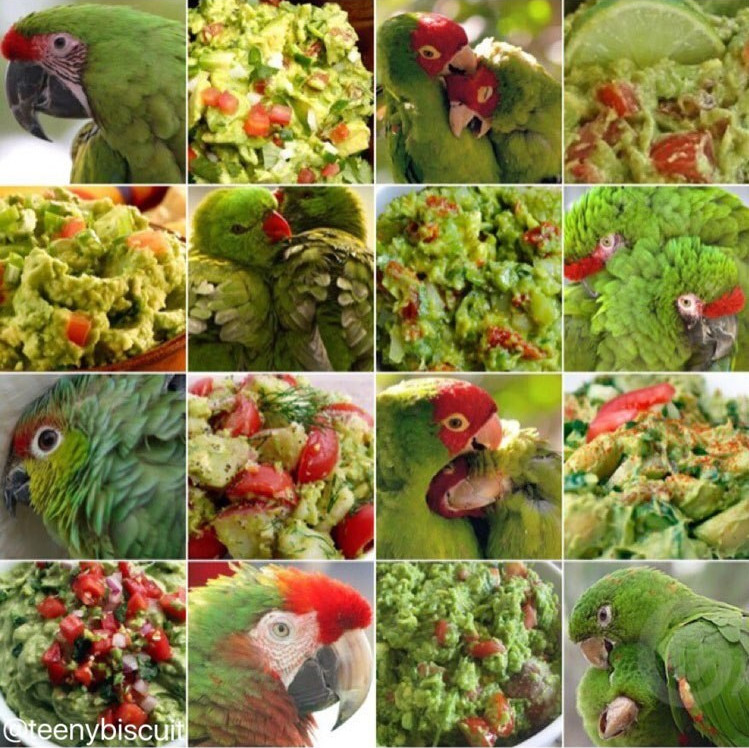
\includegraphics[width=0.3\textwidth]{guacamole}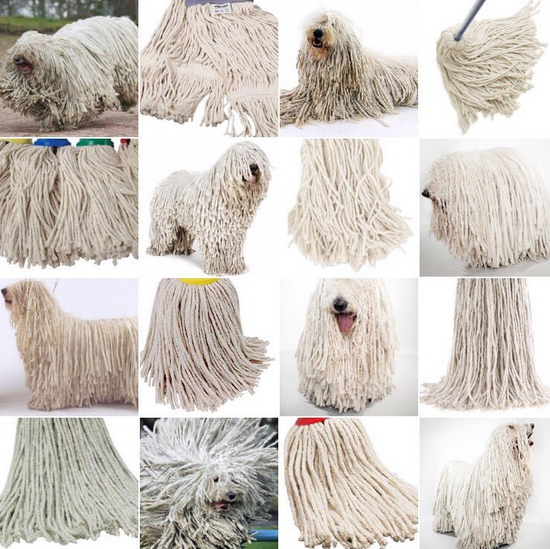
\includegraphics[width=0.3\textwidth]{sheep}
  
  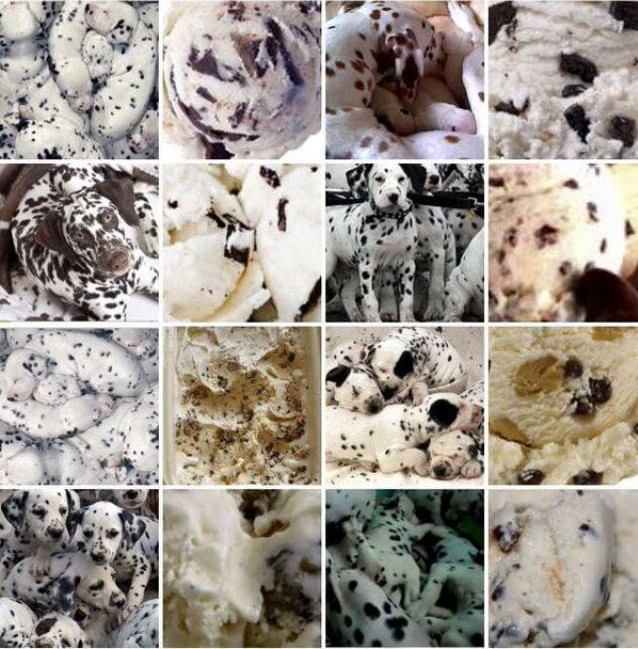
\includegraphics[width=0.3\textwidth]{ice_cream}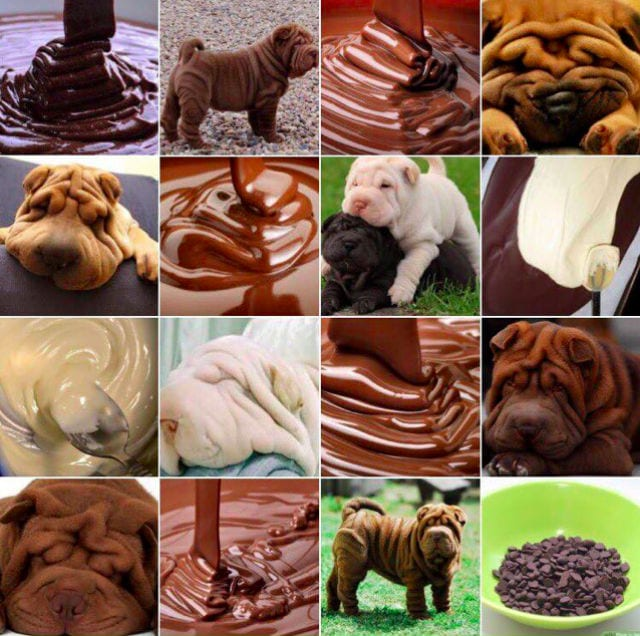
\includegraphics[width=0.305\textwidth]{chocolate}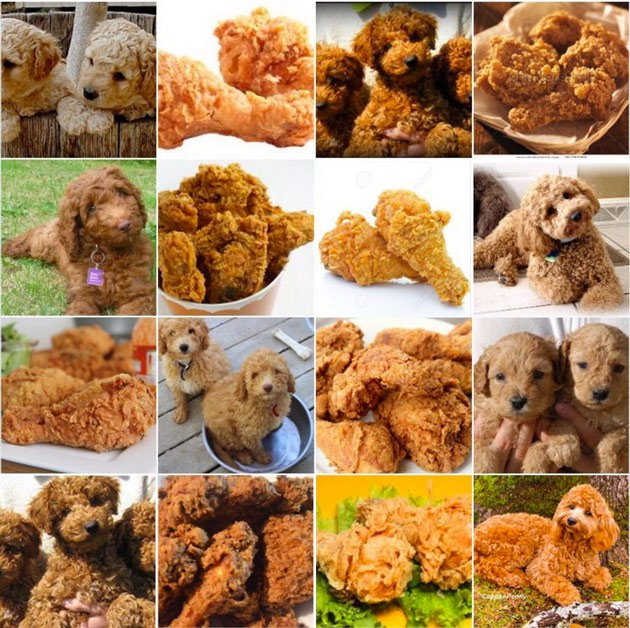
\includegraphics[width=0.305\textwidth]{fried_chicken}
  \caption{Various entries from the ``animal or things'' meme, as found on the
  internet.}
\end{figure}

\end{frame}

% ------------------------------------------------------------------------------

\begin{frame}{Oceanographic examples}


\end{frame}

% ------------------------------------------------------------------------------

\begin{frame}{Oceanographic examples}


\end{frame}

% ------------------------------------------------------------------------------

\begin{frame}{Oceanographic examples}


\end{frame}

% ------------------------------------------------------------------------------

\begin{frame}{Oceanographic examples}


\end{frame}

% ------------------------------------------------------------------------------

\begin{frame}{Oceanographic examples}


\end{frame}

% ------------------------------------------------------------------------------

\begin{frame}{Example: Argo}

\parbox{0.55\textwidth}{
\begin{itemize}
  \item A \structure{CTD} gets
  \item[] $\to$ conductivity to get $S$
  \item[] $\to$ temperature for $T$
  \item[] $\to$ it really measures $p$ to get depth
  \item[] $\to$ can put other sensors on (e.g. pH, oxygen, etc.)
  \item[]
  \item \structure{argo} system consists of CTDs that floats around the ocean
\end{itemize}
}\hspace*{3mm}\parbox{0.38\textwidth}{
\begin{figure}
  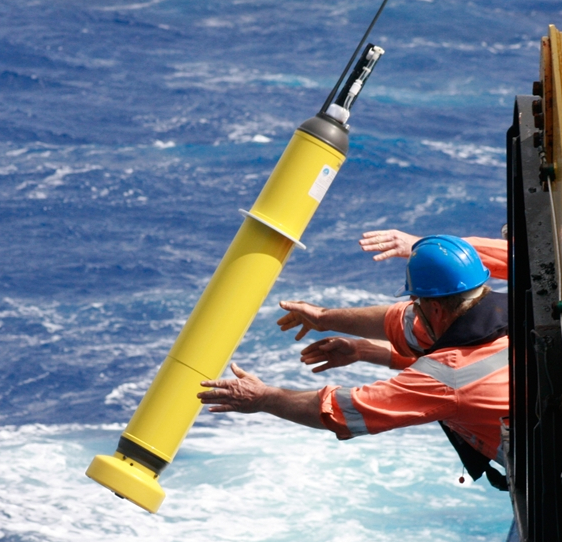
\includegraphics[width=0.38\textwidth]{argo_float}
  \caption{An Argo float being thrown off a ship. Image from NOAA.}
\end{figure}
}

\end{frame}

% ------------------------------------------------------------------------------

\begin{frame}{Example: Argo}

\begin{figure}
  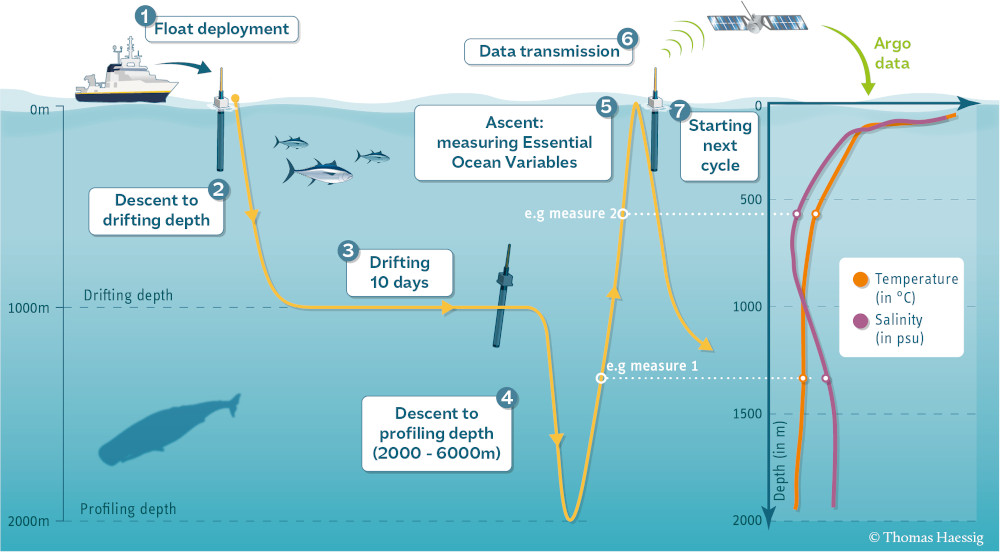
\includegraphics[width=\textwidth]{float_cycle_1}
  \caption{Argo float cycle schematic. From \texttt{argo.ucsd.edu}}
\end{figure}

\end{frame}

% ------------------------------------------------------------------------------

\begin{frame}{Example: Argo}

\begin{figure}
  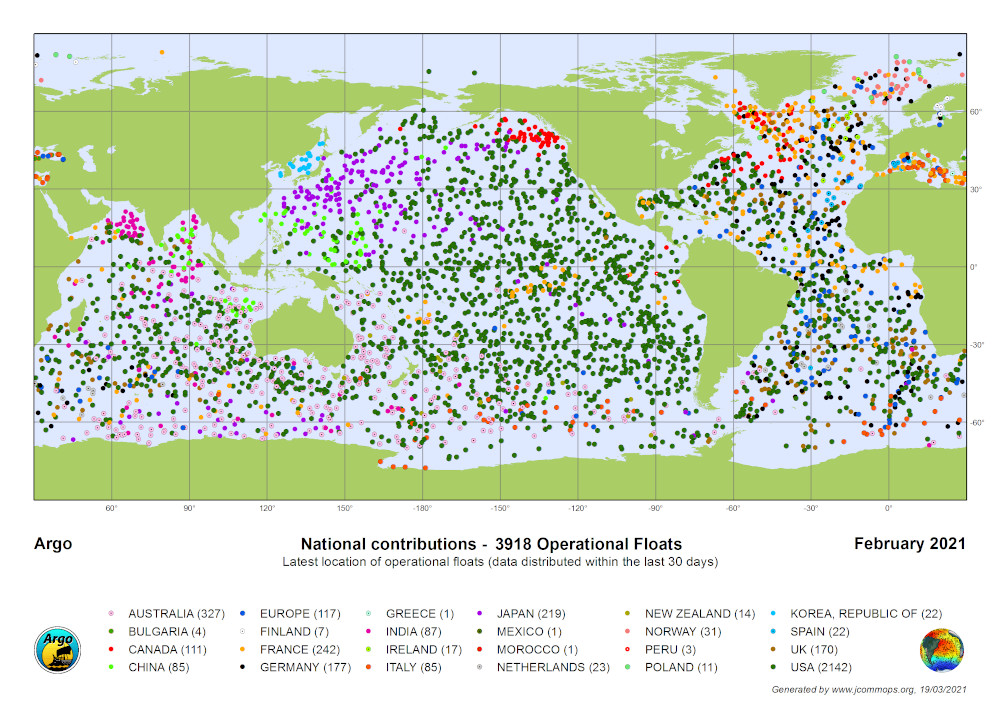
\includegraphics[width=0.9\textwidth]{argo_location}
  \caption{Argo locations as of Feb 2021. Note the dots are enhanced in size, so
  coverage is not as dense as it seems. From \texttt{argo.ucsd.edu}}
\end{figure}

\end{frame}

% ------------------------------------------------------------------------------

\begin{frame}{Example: Argo}

\begin{figure}
  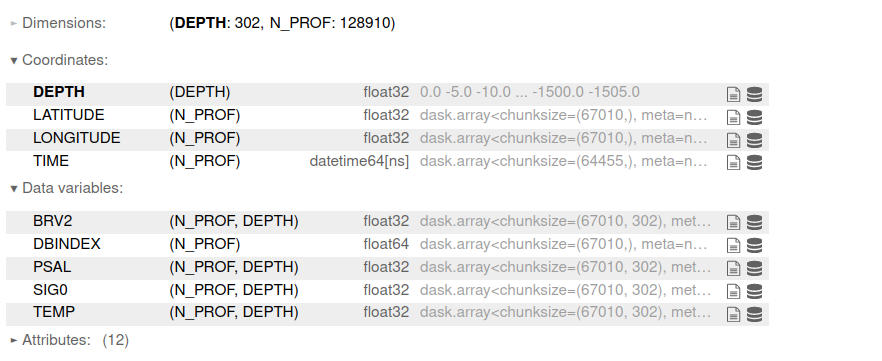
\includegraphics[width=\textwidth]{argo_dataset}
  \caption{Argo dataset in \structure{zarr} format opened as a xarray object.}
\end{figure}

\begin{itemize}
  \item argo data to be downloaded given in \structure{zarr} format
  \item[] $\to$ need \texttt{zarr} package, can open data through
  \texttt{xarray}
  \item[] $\to$ \structure{ungridded} data here
  \item[] $\to$ see also \texttt{argopy} package
\end{itemize}

\end{frame}

% ------------------------------------------------------------------------------

\begin{frame}{Example: Argo}

\begin{figure}
  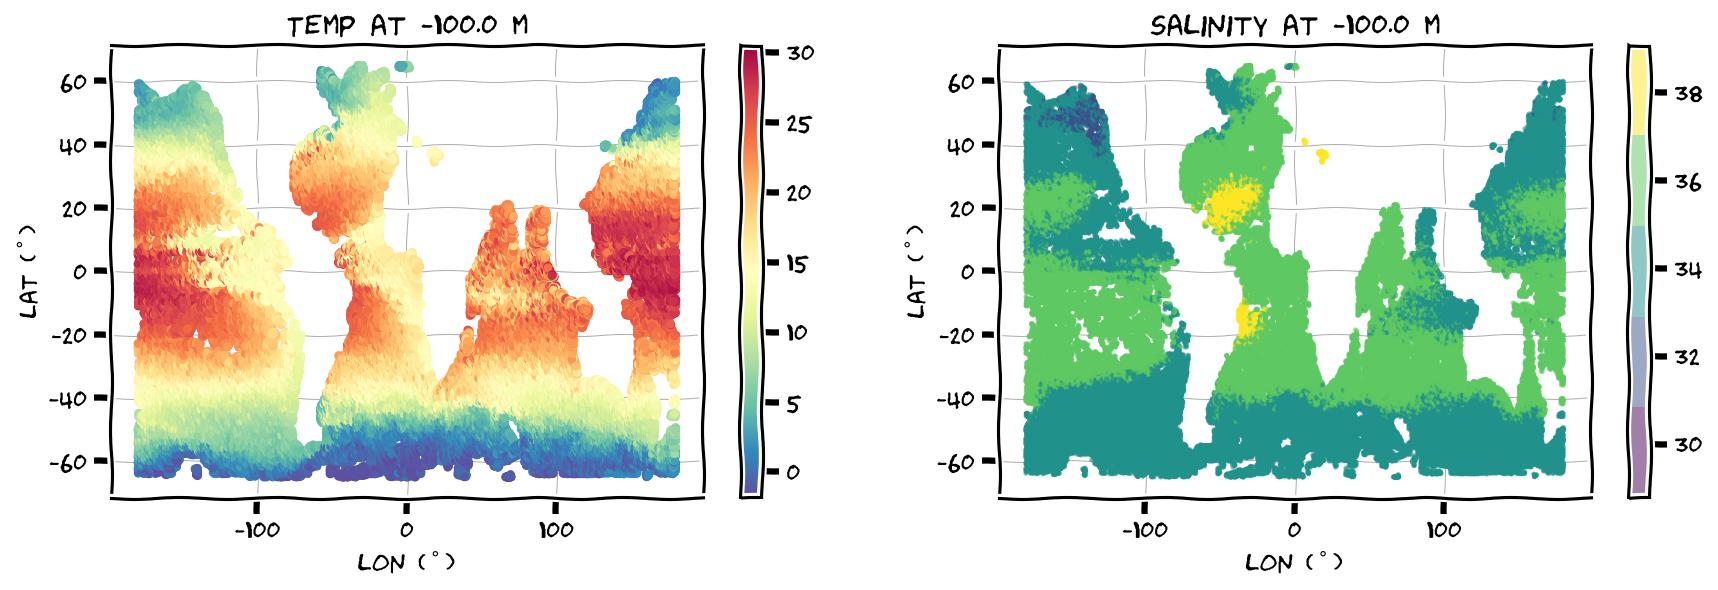
\includegraphics[width=\textwidth]{argo_data_temp_sal}
  \caption{Argo (in-situ) temperature and (practical) salinity at some fixed
  depth as a scatter plot coloured by data entry.}
\end{figure}

\begin{itemize}
  \item ungridded data, each point is an entry
  \item[] $\to$ scatter plot, with dot coloured by data
\end{itemize}

\end{frame}

% ------------------------------------------------------------------------------

\begin{frame}{Clustering}

\begin{itemize}
  \item we know different watermasses have different properties
  \item[] $\to$ e.g. NADW is more salty
  \item[] $\to$ \structure{unsupervised learning}?
\end{itemize}

\begin{figure}
  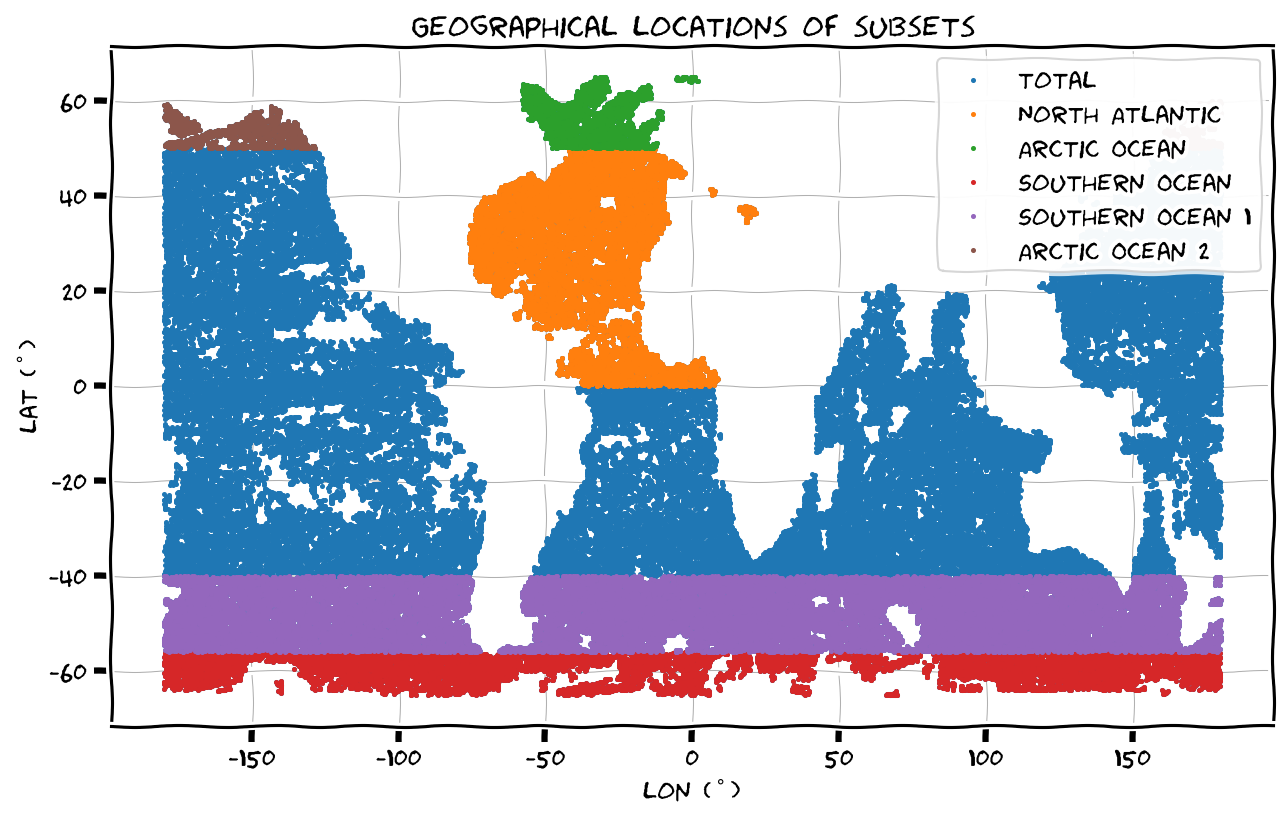
\includegraphics[width=0.6\textwidth]{argo_data_cluster}
  \caption{Artificial clustering.}
\end{figure}

\end{frame}

% ------------------------------------------------------------------------------

\begin{frame}{Clustering}

\begin{itemize}
  \item we know different watermasses have different properties
  \item[] $\to$ e.g. NADW is more salty
  \item[] $\to$ \structure{unsupervised learning}?
\end{itemize}

\begin{figure}
  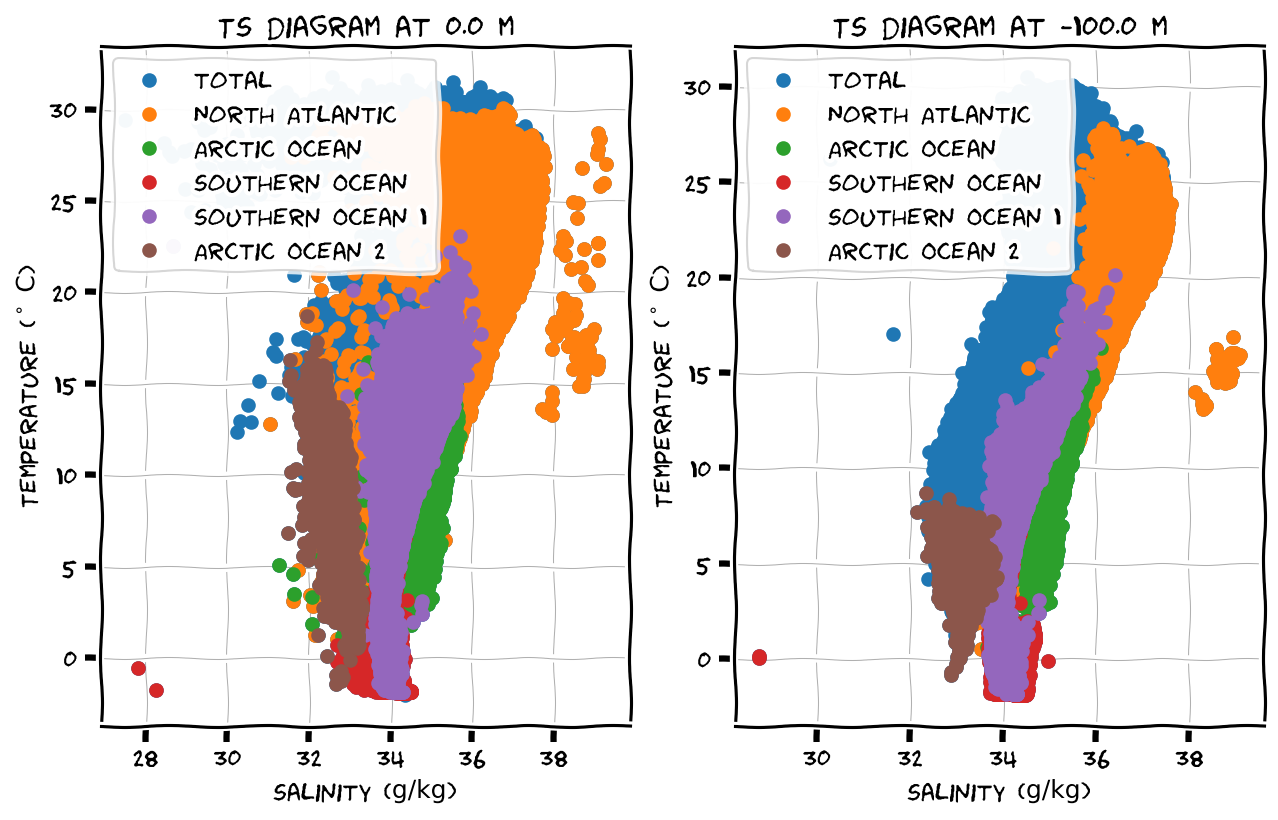
\includegraphics[width=0.8\textwidth]{argo_data_cluster_TS}
  \caption{Artificial clustering as above, but in $TS$-diagram.}
\end{figure}

\end{frame}

% ------------------------------------------------------------------------------

\begin{frame}{Clustering}

\parbox{0.5\textwidth}{
\begin{itemize}
  \item one example is \structure{$k$-means}
  \item[] $\to$ partition data and find means
  \item[] $\to$ move partitions slightly and compute new means
  \item[] $\to$ iterate on partitions such that distance to partition means are
  minimised {\tiny (finds \structure{local minimums})}
\end{itemize}
}\parbox{0.5\textwidth}{
\begin{figure}
  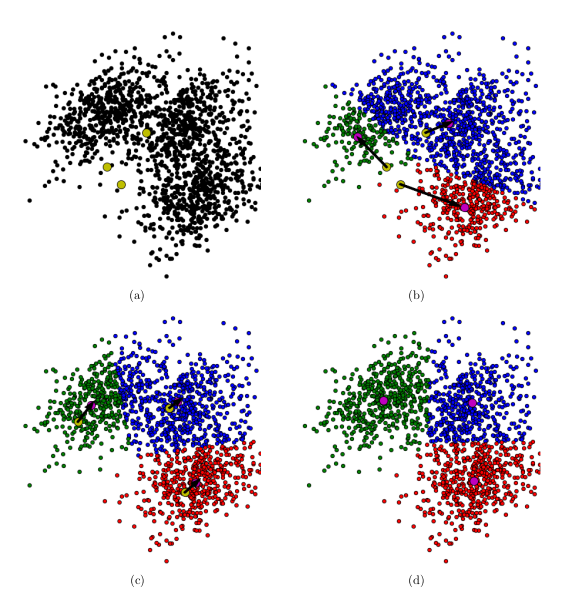
\includegraphics[width=0.5\textwidth]{k_means}
  \caption{Demonstration of $k$-means algorithm. Diagram taken from Machine
  Learning course of Christoph Haase and Varun Kanade at University of Oxford.}
\end{figure}
}

\end{frame}

% ------------------------------------------------------------------------------

\begin{frame}{Clustering}

\begin{itemize}
  \item example where $k$-means can fail
\end{itemize}

\begin{figure}
  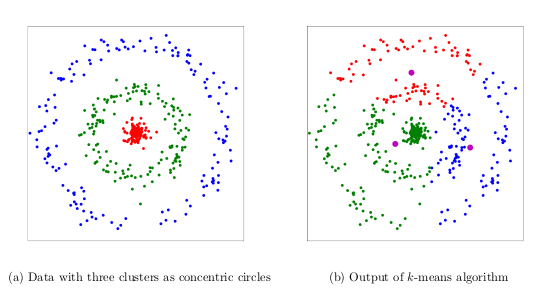
\includegraphics[width=0.7\textwidth]{k_means_fail}
  \caption{Demonstration of failure of $k$-means algorithm. Diagram taken from
  Machine Learning course of Christoph Haase and Varun Kanade at University of
  Oxford.}
\end{figure}

\end{frame}

% ------------------------------------------------------------------------------

\begin{frame}{Clustering}

\begin{figure}
  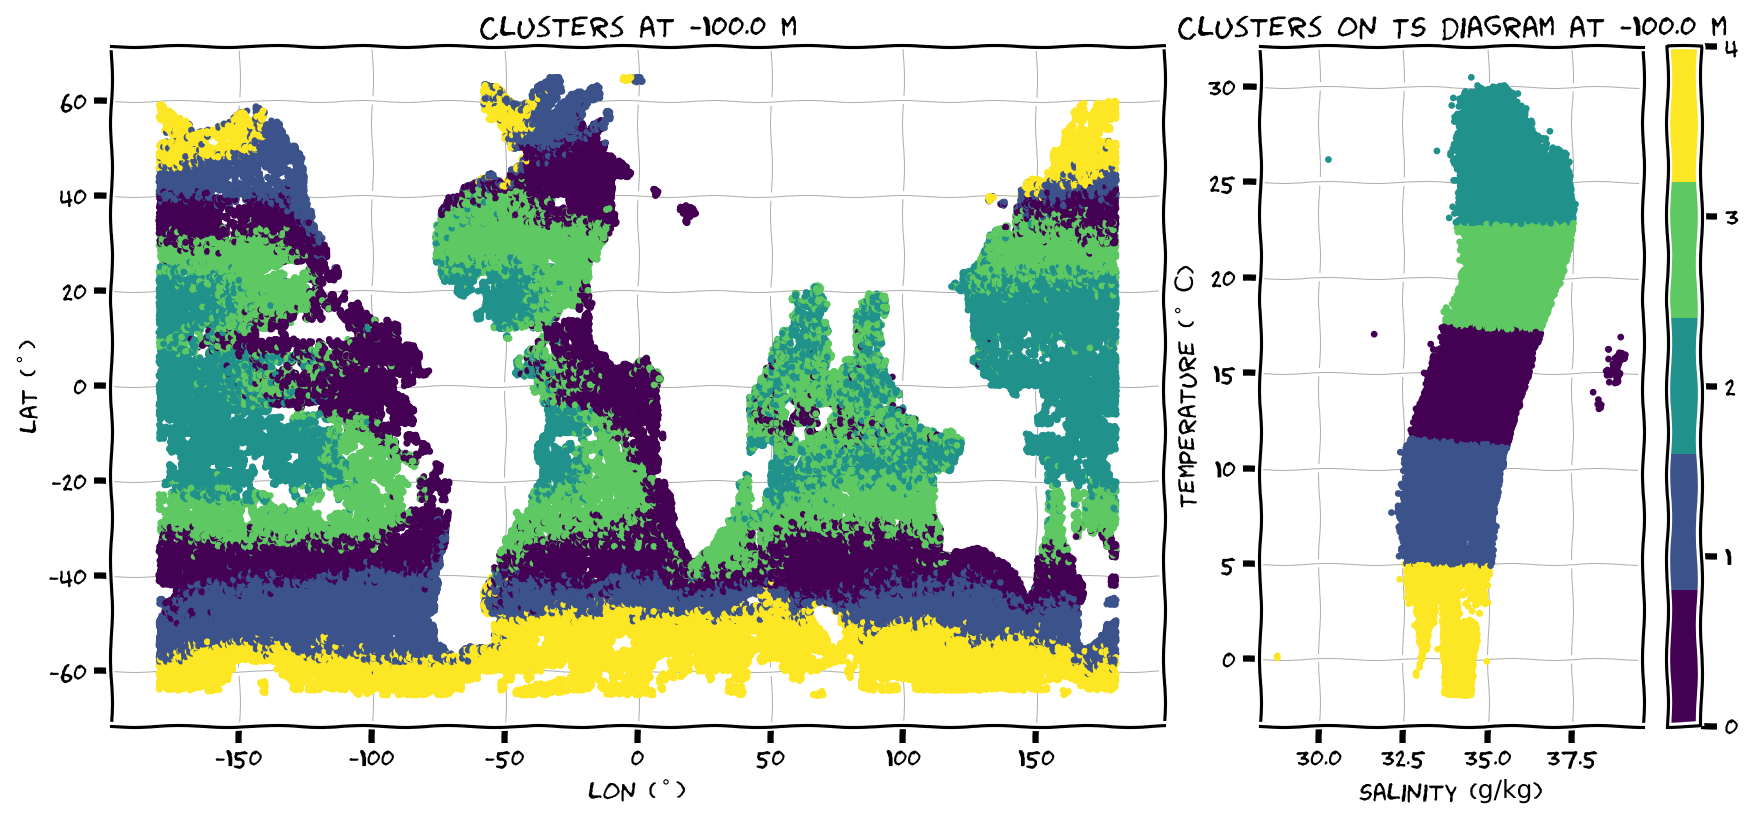
\includegraphics[width=\textwidth]{argo_data_Kmean}
  \caption{Clustering from $k$-means algorithm.}
\end{figure}

\begin{itemize}
  \item $k$-means in $TS$-space really
  \item some physical rationalisation possible
  \item[]
  \item[!!!] didn't standardise data here {\tiny (probably should have)}
\end{itemize}

\end{frame}

% ------------------------------------------------------------------------------

\begin{frame}{Clustering}

\begin{figure}
  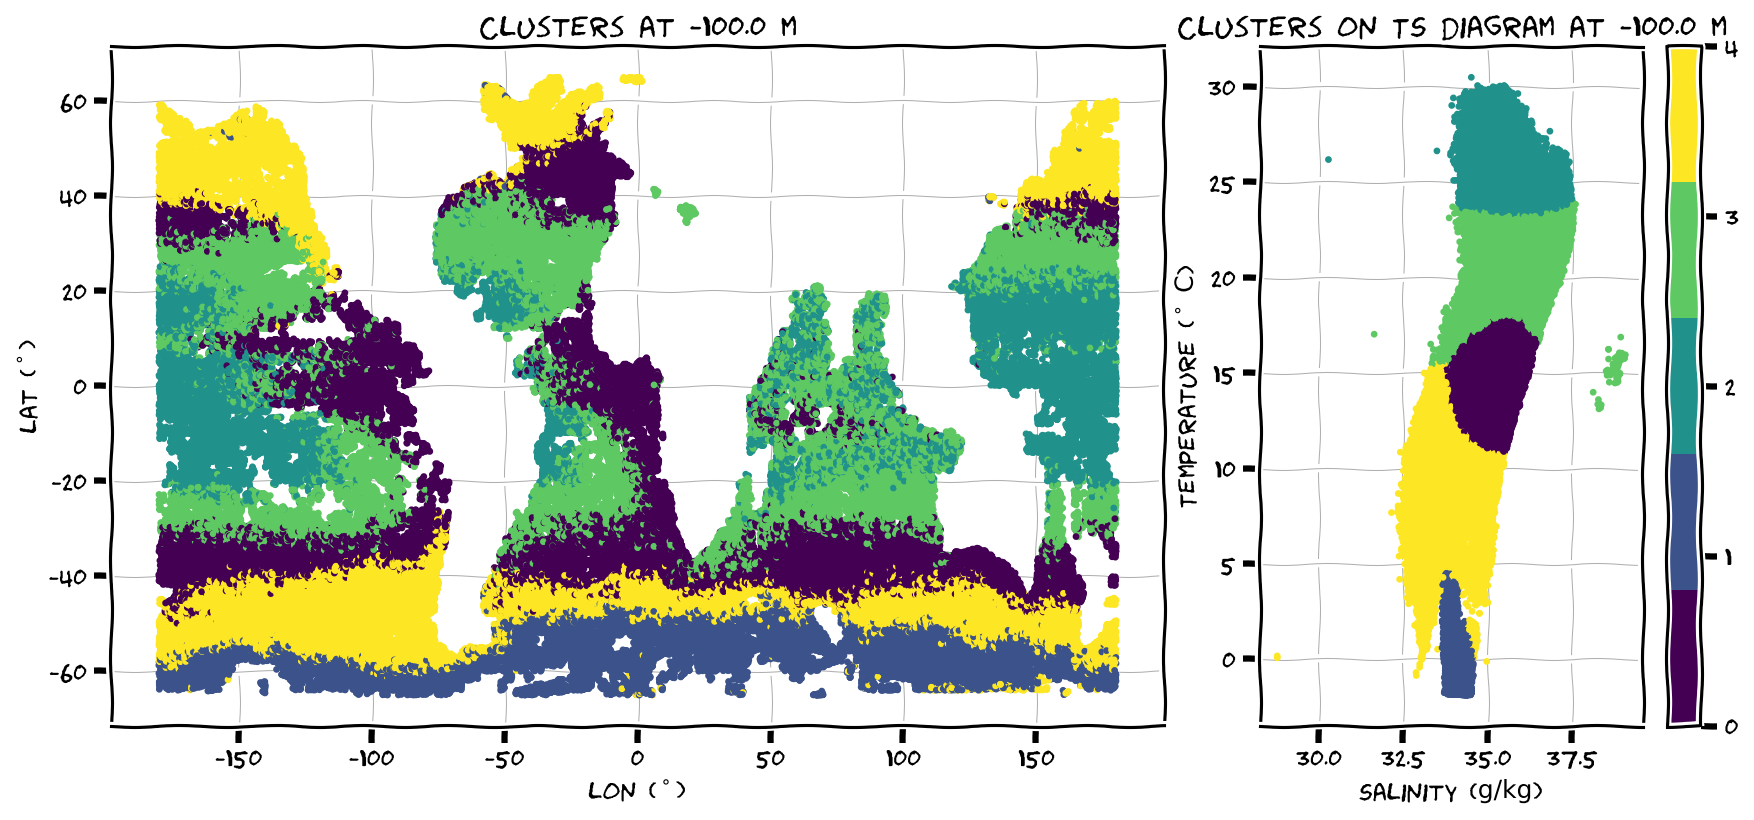
\includegraphics[width=\textwidth]{argo_data_GMM}
  \caption{Clustering from \structure{Gaussian Mixture Model}.}
\end{figure}

\begin{itemize}
  \item similar to above but with some subtle differences
  \item GMM used in oceanography before {\tiny (e.g. Jones \emph{et al.}, 2019,
  in Southern Ocean)}
  \item[]
  \item[!!!] didn't standardise data here {\tiny (probably should have)}
\end{itemize}

\end{frame}

% ------------------------------------------------------------------------------

\begin{frame}{Neural Network}

\begin{itemize}
  \item suppose we want to predict salinity from temperature, i.e.
  \structure{prediction}/\structure{reconstruction}
  \item[] $\to$ more for demonstration really...
  \item[] $\to$ split data first (\texttt{sklearn.train\_test\_split})
\end{itemize}

\begin{figure}
  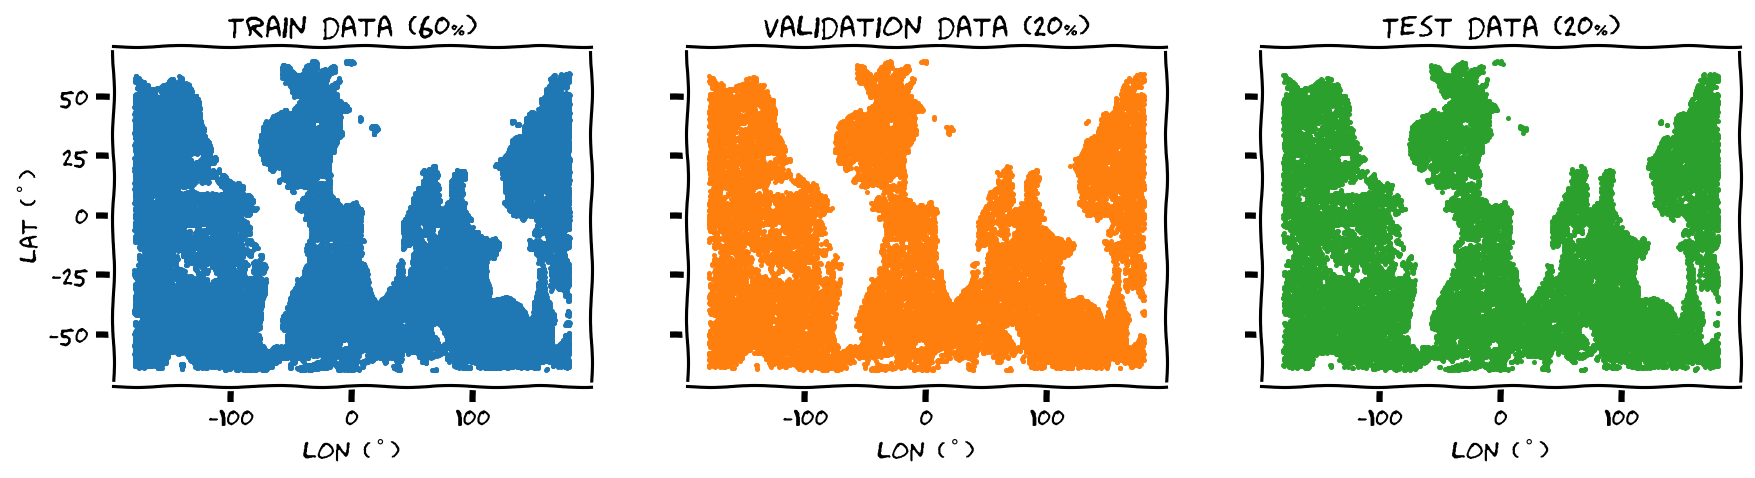
\includegraphics[width=\textwidth]{argo_data_train}
  \caption{Splitting of argo data into training:validation:test as 60:20:20.}
\end{figure}

\end{frame}

% ------------------------------------------------------------------------------

\begin{frame}{Neural Network}

\begin{itemize}
  \item linear regression?
  \item[] $\to$ standardise data
  \item[] $\to$ train with training data {\tiny (could in principle use everything)}
\end{itemize}

\begin{figure}
  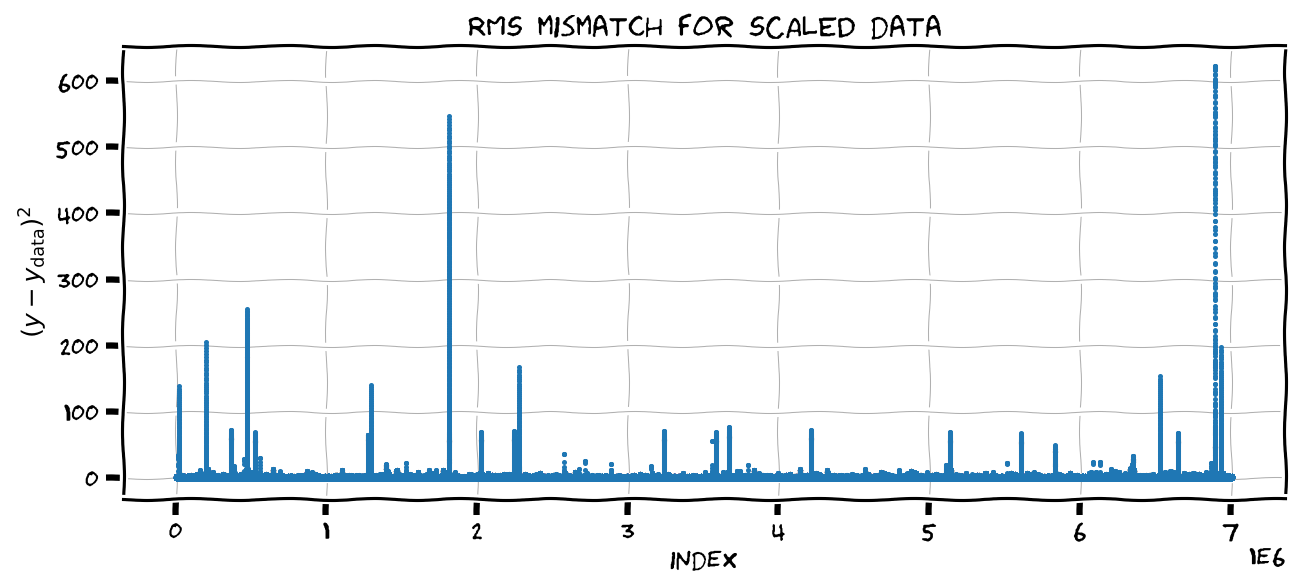
\includegraphics[width=\textwidth]{argo_data_train_linreg_RMS}
  \caption{Root-mean-square loss against index for scaled data, so anything
  larger than 1 is pretty bad.}
\end{figure}

\end{frame}

% ------------------------------------------------------------------------------

\begin{frame}{Neural Network}

\parbox{0.3\textwidth}{
\begin{figure}
  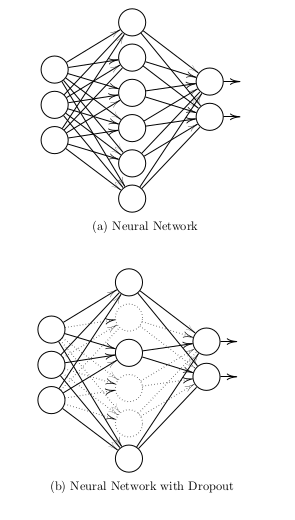
\includegraphics[width=0.3\textwidth]{network_schematic_vert}
  \caption{Schematic of neural network. Diagram adapted from Machine Learning
  course of Christoph Haase and Varun Kanade at University of Oxford.}
\end{figure}
}\parbox{0.7\textwidth}{
\begin{itemize}
  \item a \structure{neural network} has
  \item[] $\to$ \structure{nodes} containing features or transformation rules
  \item[] $\to$ \structure{links} linking the nodes
  \item[] $\to$ \structure{weights} tagged with links specifying weighting or
  transition probability going from one node to another
  \item simple case would be adjusting weights to minimise the mismatch / loss
  function
  \item[] $\to$ could in principle adjust features in nodes etc.
  \item[] $\to$ \structure{drop off} procedure as a stabiliser
\end{itemize}
}

\end{frame}

% ------------------------------------------------------------------------------

\begin{frame}{Neural Network}

\begin{itemize}
  \item train model with training and validation data
  \item[] $\to$ data has been standardised here
  \item model trained over 30 \structure{epochs}
  \item[] $\to$ think 30 complete passes/iterations
\end{itemize}

\begin{figure}
  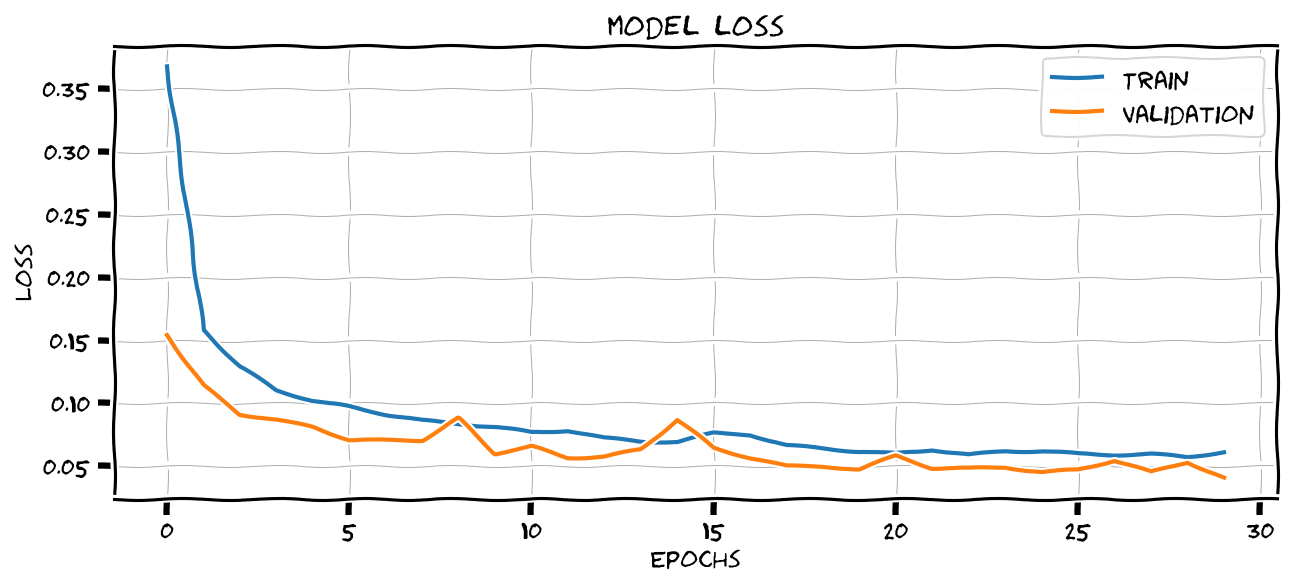
\includegraphics[width=\textwidth]{argo_data_neural_network}
  \caption{RMS loss against epoch. Note the RMS loss is not zero (and we don't
  expect it to be).}
\end{figure}

\end{frame}

% ------------------------------------------------------------------------------

\begin{frame}{Neural Network}

\begin{itemize}
  \item model takes an input depth varying {\tiny in-situ} temperature and
  returns a salinity profile
  \item[] $\to$ three random realisations below, with scaling inverted
\end{itemize}

\begin{figure}
  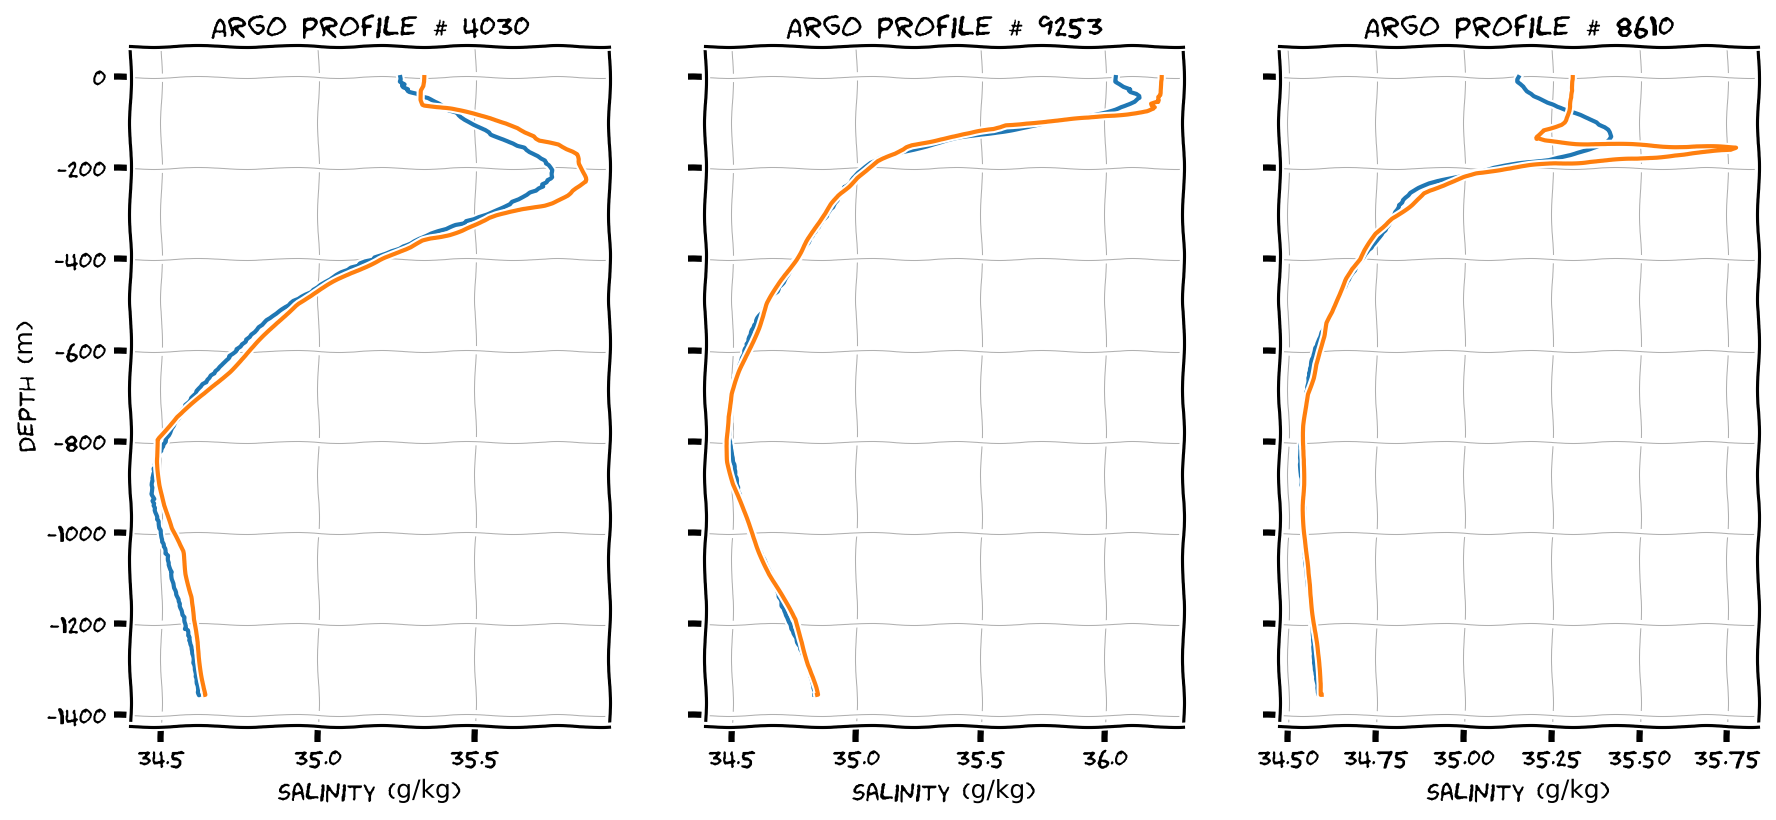
\includegraphics[width=\textwidth]{argo_data_neural_network_predict}
  \caption{Three examples of using the trained neural network.}
\end{figure}

\end{frame}

% ------------------------------------------------------------------------------

\begin{frame}{Neural Network}

\begin{figure}
  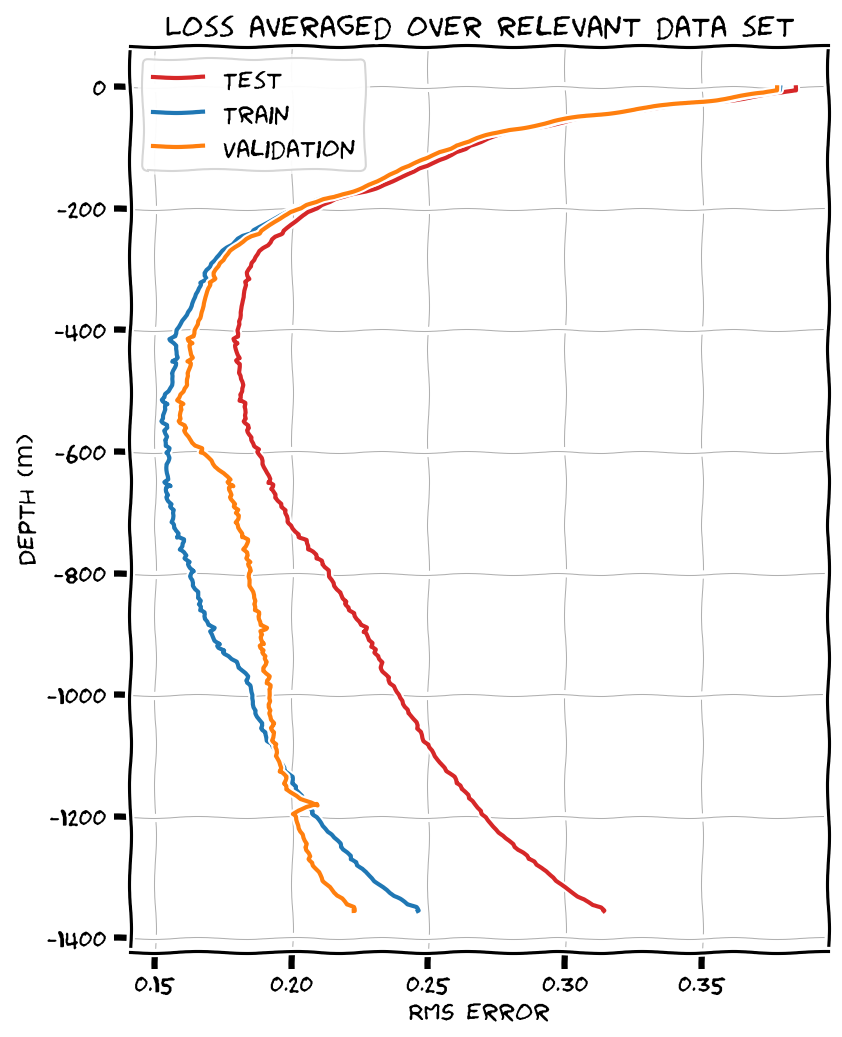
\includegraphics[width=0.3\textwidth]{argo_data_neural_network_RMS}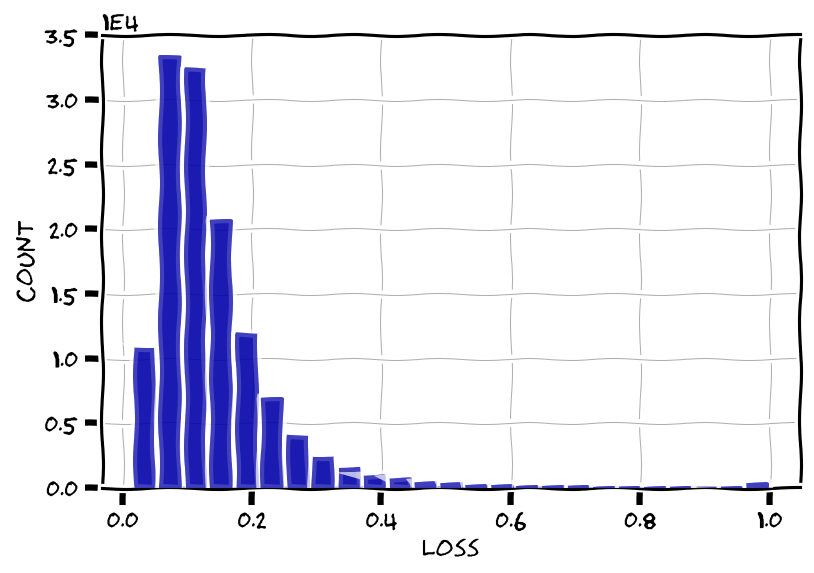
\includegraphics[width=0.5\textwidth]{argo_data_neural_network_RMS_historgram} 
  
  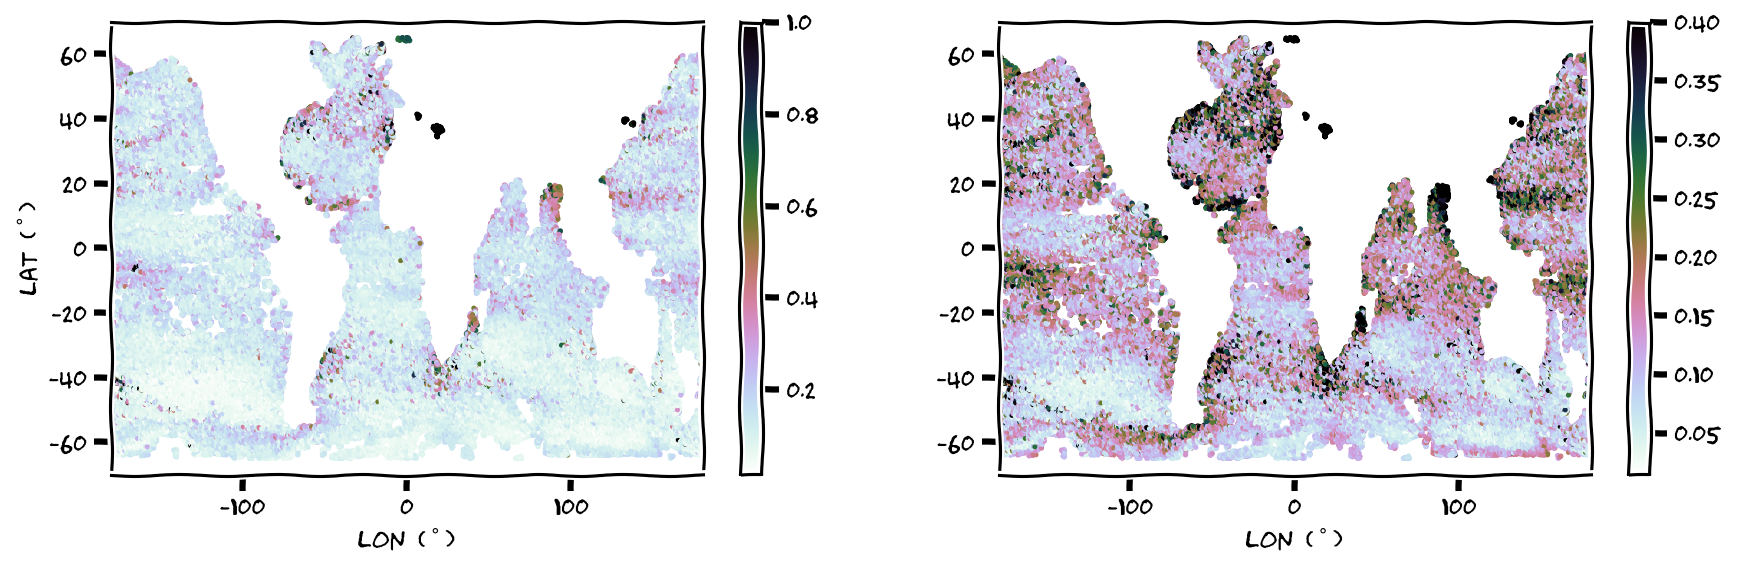
\includegraphics[width=0.9\textwidth]{argo_data_neural_network_loss_spatial}
  \caption{Some summary plots of the loss.}
\end{figure}

\end{frame}

% ------------------------------------------------------------------------------

\begin{frame}{Neural Network}

\begin{figure}
  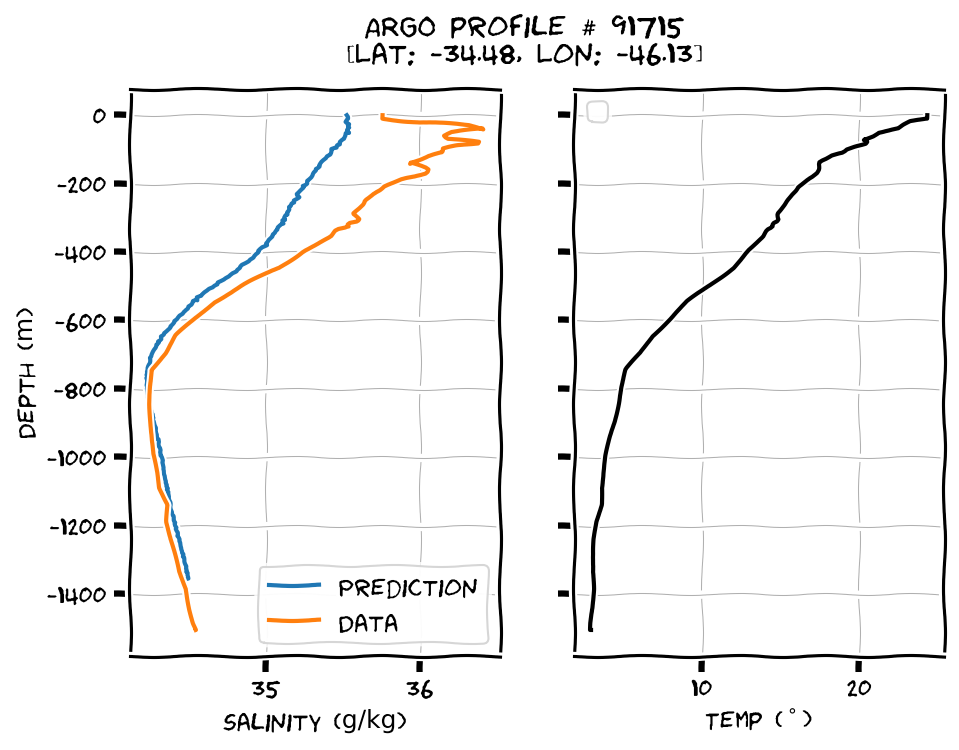
\includegraphics[width=0.8\textwidth]{argo_data_neural_network_bad_case}
  \caption{Example of a case with particularly high error.}
\end{figure}

\end{frame}

% ------------------------------------------------------------------------------

\begin{frame}{Jupyter notebook}

bonus Jupyter notebook {\tiny (with thanks to Fei Er)} to get some code practise

\medskip

\parbox{0.45\textwidth}{
\begin{itemize}
  \item different ways of reading the argo data
  \item different algorithms to try
  \item different questions to ask
  \item different features to add
  \item[] $\to$ those based on \structure{topology}?
  \item $\ldots$
\end{itemize}
}\parbox{0.55\textwidth}{
\begin{figure}
  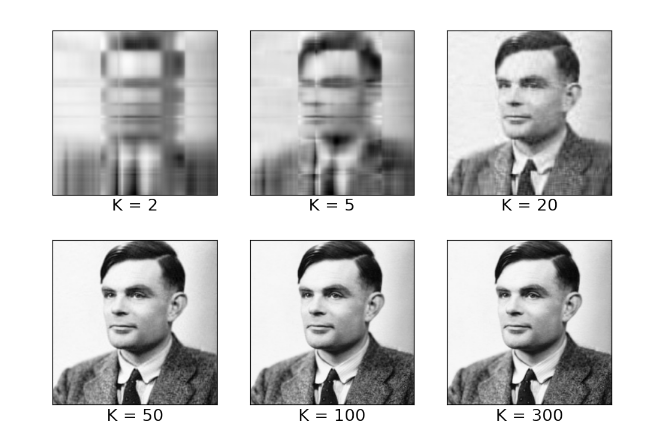
\includegraphics[width=0.55\textwidth]{turing_PCA}
  \caption{Image reconstruction: Neural network with data from PCA?}
\end{figure}
}

\end{frame}

% ------------------------------------------------------------------------------


  

\end{document}


